\documentclass[12pt,a4paper]{article}
\usepackage[margin=2cm]{geometry}
\usepackage{xeCJK}
\usepackage{fontspec}
\setCJKmainfont{Noto Serif CJK TC}[Script=CJK]
\usepackage{amsmath,amssymb}
\usepackage{graphicx}
\usepackage{fancyhdr}
\setlength{\headheight}{14.5pt}
\addtolength{\topmargin}{-2.5pt}
\usepackage{hyperref}
\usepackage{listings}
\usepackage{enumitem}
\usepackage{titlesec}
\usepackage{caption}
\usepackage{indentfirst}
\usepackage{booktabs}
\usepackage{longtable}
\usepackage{multirow}
\usepackage{array}
\usepackage{tabularx}
\usepackage{float}
\usepackage{minted}
\setlength{\parindent}{2em}
\pagestyle{fancy}
\fancyhf{}
\cfoot{\thepage}
\linespread{1.3}
\setminted{
    linenos,                % 行號
    frame=lines,            % 上下框線
    framesep=5pt,           % 程式碼與邊框距離
    numbersep=8pt,          % 行號與程式碼距離
    fontsize=\scriptsize,   % 字體大小
    breaklines,             % 自動換行
    tabsize=4,              % tab 寬度
    rulecolor=\color{black},% 框線顏色
    xleftmargin=1.5em       % 左側縮排
}

\title{Time Frequency Analysis and Wavelet Transforms Homework 2}
\author{B12508026戴偉璿}
\date{\today}

\begin{document}

\maketitle

\lhead{TFW HW 2}
\rhead{B12508026戴偉璿}

\begin{enumerate}

%=====================================================================
\item
\textbf{Advantages:} 

Since each $X(n\Delta t,m\Delta f)$ is obtained from $X((n-1)\Delta t,m\Delta f)$ by removing one sample and adding one sample, the recursive method has the lowest complexity, i.e., $O(TF)$, where $T$ and $F$ are the numbers of sampling points on the $t$- and $f$-axes.  

Moreover, only the required $F$ frequency points are computed, while the FFT-based method always computes all $N$ points.

\textbf{Disadvantages:} 

It works only for the rec-STFT, and the constraints of the FFT-based method still hold, i.e., $\Delta t\Delta f$ must be the reciprocal of an integer $N$ with $N\ge 2Q+1$, and $\Delta t<1/(2\Omega)$.

Also, the round-off error accumulates along the $t$-axis.

%=====================================================================
\item Since $x(t)=\cos(6\pi t+1)$ is real, $x^*(t)=x(t)$ and $x\!\left(t\pm\tfrac\tau2\right)=\cos(6\pi t\pm3\pi\tau+1)$. 

Using $\cos A\cos B=\frac12[\cos(A-B)+\cos(A+B)]$ and $\int e^{-j2\pi(f-f_0)\tau}d\tau=\delta(f-f_0)$.

We have
\begin{align*}
W_x(t,f)&=\int_{-\infty}^{\infty}x\!\left(t+\tfrac{\tau}{2}\right)x^*\!\left(t-\tfrac{\tau}{2}\right)e^{-j2\pi f\tau}\,d\tau\\
&=\int_{-\infty}^{\infty}\cos(6\pi t+3\pi\tau+1)\cos(6\pi t-3\pi\tau+1)\,e^{-j2\pi f\tau}d\tau\\
&=\int_{-\infty}^{\infty}\Big[\tfrac12\cos(6\pi\tau)+\tfrac12\cos(12\pi t+2)\Big]e^{-j2\pi f\tau}d\tau\\
&=\int_{-\infty}^{\infty}\Big[\tfrac14e^{j6\pi\tau}+\tfrac14e^{-j6\pi\tau}+\tfrac12\cos(12\pi t+2)\Big]e^{-j2\pi f\tau}d\tau\\
&=\tfrac14\delta(f-3)+\tfrac14\delta(f+3)+\tfrac12\cos(12\pi t+2)\,\delta(f)
\end{align*}

%=====================================================================
\item The WDF has cross terms when the signal has more than one component, or the phase has an order larger than 2.

With these two conditions , we check each case:
\begin{enumerate}[label=(\alph*)]
  \item $\delta(-\pi t)$: \textbf{No.} $\delta(-\pi t)=\frac1\pi\delta(t)$ is a single component, and $W_x(t,f)=\frac{1}{\pi^2}\delta(t)$.

  \item $\exp(-\pi t^4)$: \textbf{No.} It is a single real pulse with zero phase, so its WDF is a single lobe around $(t,f)=(0,0)$.

  \item $\exp(j\pi t^4)$: \textbf{Yes.} The phase has order 4:
  \[
  x(t+\tfrac\tau2)x^*(t-\tfrac\tau2)=e^{j2\pi(2t^3)\tau}\,e^{j\pi t\tau^3}.
  \]
  The extra factor $e^{j\pi t\tau^3}$ spreads $\delta(f-2t^3)$ into oscillating interference.

  \item $\cos(-\pi t^2)$: \textbf{Yes.} $\cos(\pi t^2)=\frac12\big[e^{j\pi t^2}+e^{-j\pi t^2}\big]$ has two components, so
  \[
  W_x(t,f)=\tfrac14\big[\delta(f-t)+\delta(f+t)\big]+\underbrace{\tfrac{\sqrt2}{2}\cos\!\big(2\pi(t^2-f^2)+\tfrac\pi4\big)}_{\text{cross term}}.
  \]

  \item A music signal: \textbf{Yes.} It contains many notes and harmonics, i.e., many components, and every pair of components produces cross terms.
\end{enumerate}

\noindent Therefore, (c), (d), and (e) have the cross-term problem.
%=====================================================================
\item
\begin{enumerate}[label=(\alph*)]
  \item \textbf{Cohen's class distribution.} With the ambiguity function (AF)
  \[
  A_x(\tau,\eta)=\int x(t+\tfrac\tau2)\,x^*(t-\tfrac\tau2)\,e^{-j2\pi t\eta}dt,
  \]
  the WDF is the 2-D FT of the AF: $W_x(t,f)=\iint A_x(\tau,\eta)\,e^{j2\pi(\eta t-\tau f)}d\eta\,d\tau$. Consider $x=x_1+x_2$ with components centered at $(t_1,f_1)$ and $(t_2,f_2)$:
  \begin{itemize}
    \item The auto terms $A_{x_1}$, $A_{x_2}$ are always located near the origin of the $(\tau,\eta)$ plane, since $|A_{x_k}(\tau,\eta)|$ depends only on the shape, while the position $(t_k,f_k)$ only contributes a phase.
    \item The cross terms $A_{x_1x_2}$, $A_{x_2x_1}$ are located at $(\tau,\eta)=\pm(t_1-t_2,\,f_1-f_2)$, i.e., far from the origin when the components are separated.
  \end{itemize}
  The Cohen's class distribution
  \[
  C_x(t,f)=\iint A_x(\tau,\eta)\,\Phi(\tau,\eta)\,e^{j2\pi(\eta t-\tau f)}d\eta\,d\tau
  \]
  chooses $\Phi(\tau,\eta)$ as a low-pass function: $\Phi\approx1$ near the origin, where the auto terms are, and $\Phi\approx0$ in the region where the cross terms are. For example, the Choi-Williams kernel $\Phi(\tau,\eta)=e^{-\alpha(\eta\tau)^2}$ equals $1$ on the $\tau$- and $\eta$-axes and decays away from them. Since the cross terms at $\pm(t_1-t_2,f_1-f_2)$ are usually off the axes, they are suppressed. Thus, the auto terms are kept and the cross terms are filtered out before transforming back. ($\Phi=1$ gives the WDF.) The cost is a tradeoff: a stronger low-pass filter removes more cross terms but also blurs the auto terms.

  \item \textbf{Polynomial WDF.} It replaces $x(t+\frac\tau2)x^*(t-\frac\tau2)$ by a product of more terms:
  \[
  W_x(t,f)=\int\prod_{l=1}^{q/2}x(t+d_l\tau)\,x^*(t-d_{-l}\tau)\,e^{-j2\pi f\tau}d\tau .
  \]
  For $x(t)=\exp\!\big(j2\pi\sum_{n=1}^{q/2+1}a_nt^n\big)$, $d_l$ are chosen such that all terms with $\tau^2,\tau^3,\ldots$ cancel and
  \[
  \prod_{l=1}^{q/2}x(t+d_l\tau)\,x^*(t-d_{-l}\tau)=\exp\!\Big(j2\pi\tau\sum_{n=1}^{q/2+1} na_nt^{n-1}\Big),
  \]
  which is linear in $\tau$. Hence $W_x(t,f)=\delta\big(f-\sum_n na_nt^{n-1}\big)$, exactly on the instantaneous frequency. Therefore, the polynomial WDF avoids the cross term when the order of the phase is no larger than $q/2+1$.
  \begin{itemize}
    \item For $q=2$, $d_1=d_{-1}=\frac12$ gives the original WDF, which can only handle a phase of order up to 2.
    \item For $q=4$, the conditions
    \[
    \textstyle\sum_l d_l+\sum_l d_{-l}=1,\quad \sum_l d_l^2-\sum_l d_{-l}^2=0,\quad \sum_l d_l^3+\sum_l d_{-l}^3=0
    \]
    cancel the $\tau^2$ and $\tau^3$ terms, so a phase of order up to 3 can be handled.
  \end{itemize}
  Thus it avoids the interference of a single component with a higher-order phase. For example, Problem 3(c) $\exp(j\pi t^4)$ has a phase of order 4, so $q\ge 6$ is required. However, the cross terms between two different components cannot be removed.

  \item \textbf{Gabor-Wigner transform.} It combines the two distributions, e.g., $D_x(t,f)=G_x(t,f)\,W_x(t,f)$, $\min\!\big(|G_x(t,f)|^2,|W_x(t,f)|\big)$, or $G_x^\alpha(t,f)\,W_x^\beta(t,f)$. The Gabor transform is linear, $G_{x_1+x_2}=G_{x_1}+G_{x_2}$, so it has no cross term: $G_x\approx0$ wherever there is no signal component, but its clarity is poor. The WDF has high clarity but cross terms. Multiplying them:
  \begin{itemize}
    \item at the cross terms of $W_x$, $G_x\approx0$, so $D_x\approx0$ and the cross terms are removed;
    \item at the auto terms, both are nonzero, and the product keeps the high clarity of the WDF.
  \end{itemize}
  For example, for $x(t)=\cos(2\pi t)$, the cross term of $W_x$ at $f=0$ is removed since $G_x(t,0)\approx0$.
\end{enumerate}


%=====================================================================
\item
\begin{enumerate}[label=(\alph*)]
  \item From large to small:
  \[
  \text{(iv) Cohen's class} \;>\; \text{(ii) Gabor-Wigner} \;>\; \text{(iii) windowed WDF} \;>\; \text{(i) rec-STFT}.
  \]

  \item The windowed WDF is
  \[
  W_x^w(t,f)=\int w(\tau)\,x(t+\tfrac\tau2)\,x^*(t-\tfrac\tau2)\,e^{-j2\pi f\tau}d\tau .
  \]
  Taking the conjugate and substituting $\tau=-u$:
  \begin{align*}
  \big[W_x^w(t,f)\big]^*&=\int w^*(\tau)\,x^*(t+\tfrac\tau2)\,x(t-\tfrac\tau2)\,e^{j2\pi f\tau}d\tau\\
  &=\int w^*(-u)\,x(t+\tfrac u2)\,x^*(t-\tfrac u2)\,e^{-j2\pi fu}du .
  \end{align*}
  Comparing with $W_x^w(t,f)$, it is real for every $x(t)$ if and only if
  \[
  \boxed{w(\tau)=w^*(-\tau)}
  \]
  Since $w(\tau)$ is usually chosen to be real, the constraint becomes $w(\tau)=w(-\tau)$, i.e., the window must be real and even.

  \item \textbf{No.} As the original WDF, it cannot distinguish $x(t)$ and $e^{j\theta}x(t)$, since the constant phase cancels in $x(t+\frac\tau2)x^*(t-\frac\tau2)$. 
  
  Moreover, the mask causes more information loss. Suppose that $w(\tau)=0$ for $|\tau|>B$. Taking the IFT along $f$ only recovers $w(\tau)x(t+\frac\tau2)x^*(t-\frac\tau2)$, so with $t_1=t+\frac\tau2$ and $t_2=t-\frac\tau2$, we only know $x(t_1)x^*(t_2)$ for $|t_1-t_2|<B$. 
  
  Therefore, if $x(t)=s_1(t)+e^{j\theta}s_2(t)$, where $s_1$ and $s_2$ are separated by a gap larger than $B$, all the products between $s_1$ and $s_2$ fall outside the mask, and the windowed WDF is the same for every $\theta$. 
\end{enumerate}

%=====================================================================
\item The code (i.e., \texttt{recSTFT.py}) is uploaded to NTU Cool, and it is written by the FFT-based method. Using the example input with $B=1$, the output is shown below.

\begin{figure}[H]
\centering
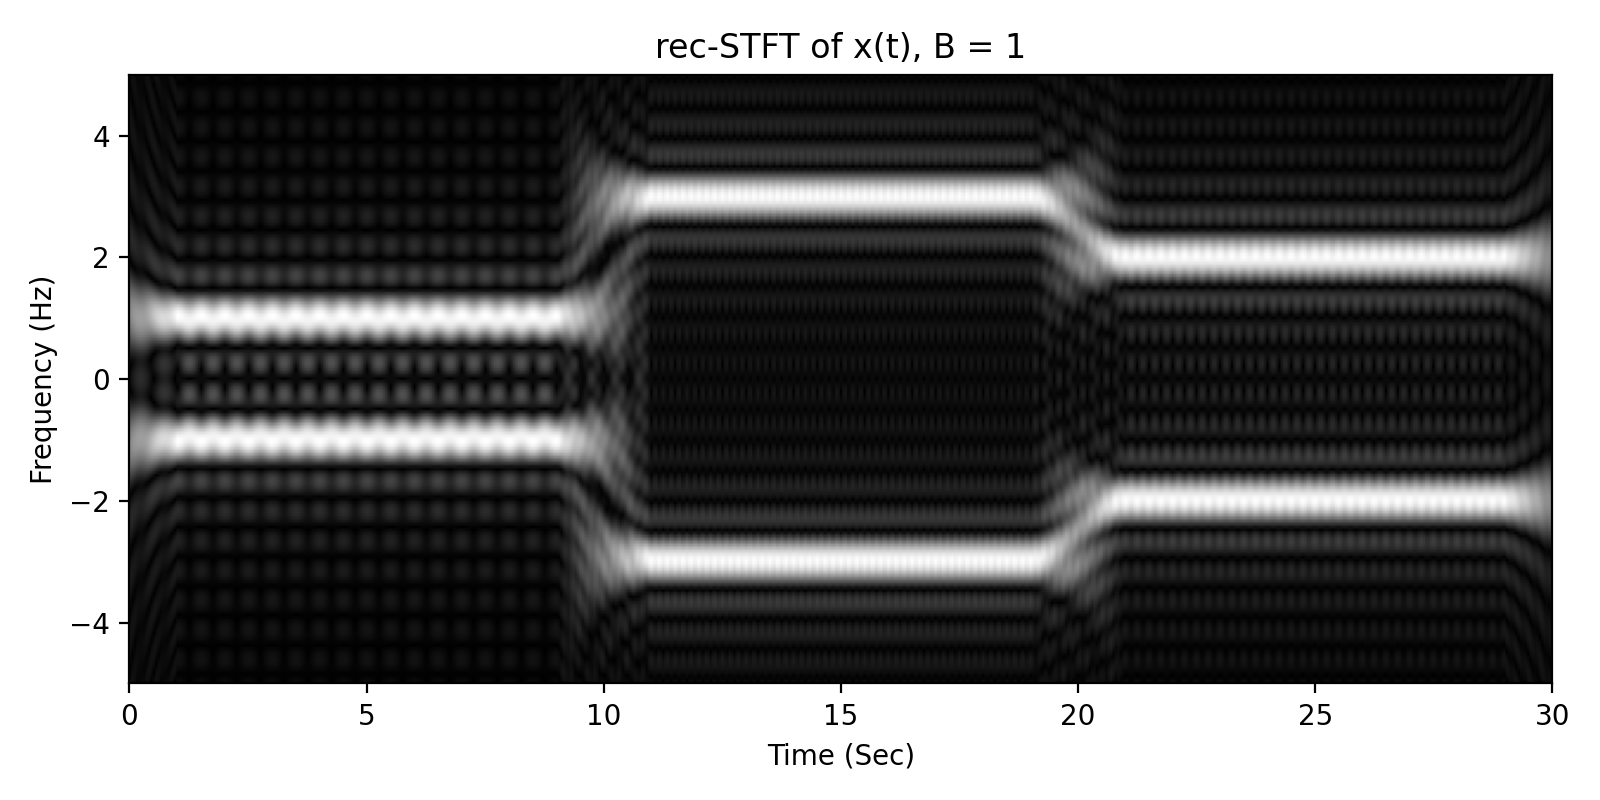
\includegraphics[width=0.9\textwidth]{recSTFT_result.png}
\caption{rec-STFT of $x(t)$ with $B=1$.}
\end{figure}

The running time is $0.0163$ s.


%=====================================================================
\item (extra) 
\begin{figure}[H]
\centering
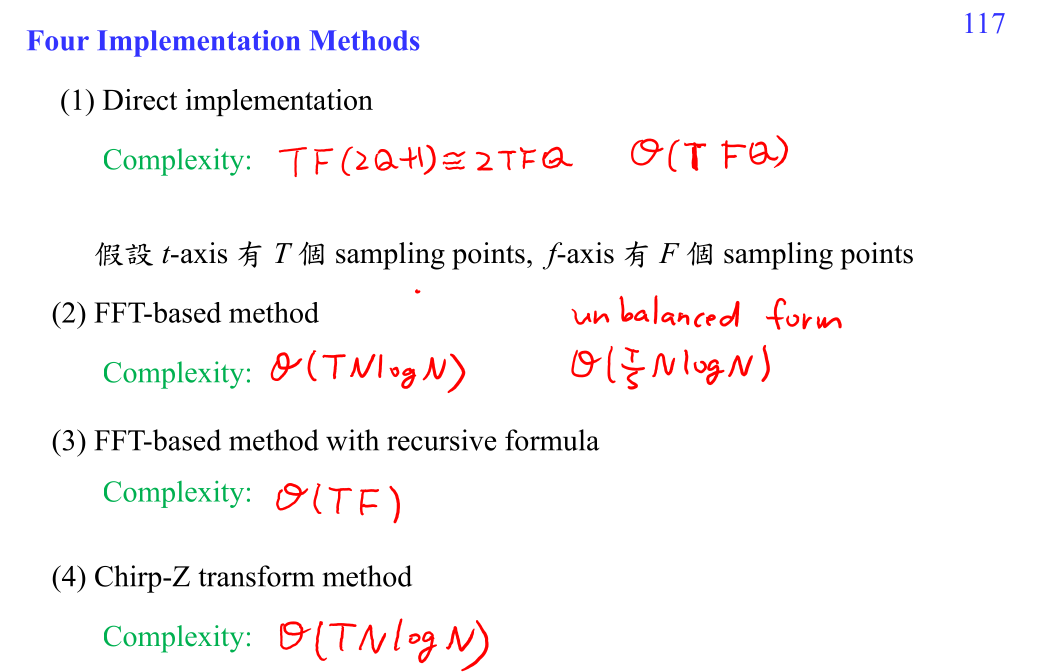
\includegraphics[width=0.9\textwidth]{extra.png}
\end{figure}

\textbf{(1) Direct implementation} and \textbf{(4) Chirp-Z transform method} can also be used in the unbalanced form besides the FFT-based method.

Let $S=\Delta_t/\Delta_\tau$ be an integer, where $\Delta_\tau$ and $\Delta_t$ are the input and output sampling intervals. If the input has $T$ points, the output $t$-axis has only $T/S$ points. In both methods, each output time is computed independently, so only these $T/S$ points need to be computed:
\begin{itemize}
  \item Direct implementation: $O\!\left(\frac{T}{S}FQ\right)$.
  \item Chirp Z transform: $O\!\left(\frac{T}{S}N\log_2N\right)$, since the chirp decomposition still holds with $\Delta_\tau\Delta_f$ in place of $\Delta_t\Delta_f$.
\end{itemize}
The recursive method gives no saving: each step is derived from the previous one, so when the window moves by $S$ samples, $S$ terms must be removed and $S$ terms added, and the complexity remains $\frac{T}{S}\cdot F\cdot 2S=O(TF)$.

\end{enumerate}

\end{document}